\documentclass[a4paper,12pt]{article}
\usepackage[utf8]{inputenc}
\usepackage[english]{babel}
\usepackage{amsmath,amssymb}
\usepackage{geometry}\geometry{margin=2.5cm}
\usepackage{enumitem}
\usepackage{booktabs}
\usepackage{tikz}
\usetikzlibrary{arrows.meta, positioning, calc, decorations.pathreplacing}
\usepackage{pgfplots}\pgfplotsset{compat=1.18}
\usepackage{tcolorbox}
\tcbuselibrary{breakable}
\usepackage{xcolor}

\newtcolorbox{merkbox}[1][]{colback=blue!5, colframe=blue!40, fonttitle=\bfseries, title={Remember}, breakable, #1}
\newtcolorbox{analogie}[1][]{colback=green!5, colframe=green!40, fonttitle=\bfseries, title={Analogy}, breakable, #1}
\newtcolorbox{begriffe}[1][]{colback=yellow!10, colframe=yellow!60!black, fonttitle=\bfseries, title={What do the terms mean?}, breakable, #1}
\newcommand{\EW}{eigenvalue}
\newcommand{\EV}{eigenvector}

\title{Explanation -- HW12: Diagonalization \& Applications}
\author{}
\date{}

\begin{document}
\maketitle

%=============================================================================
\part*{Part 1: Foundations -- explained simply}

%-----------------------------------------------------------------------------
\section*{1. What does ``diagonalizing'' mean? The right glasses}

A matrix $A$ deforms space -- usually in a complicated way (rotating \emph{and} stretching). But in HW11 we saw: there are special directions, the \textbf{eigenvectors}, that $A$ only \emph{stretches}. Diagonalizing means: look at space through the ``eigenvector glasses''. Through these glasses $A$ does nothing complicated anymore -- it just stretches each axis by its eigenvalue. That is the \textbf{diagonal matrix $D$}.

\begin{center}
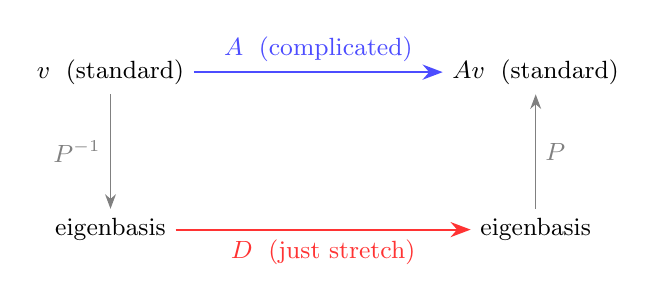
\begin{tikzpicture}[scale=1.0, >={Stealth[scale=1.1]}, every node/.style={font=\small}]
\node (vE)  at (0,2)   {$v$ \;(standard)};
\node (wE)  at (5.4,2) {$Av$ \;(standard)};
\node (vB)  at (0,0)   {eigenbasis};
\node (wB)  at (5.4,0) {eigenbasis};
\draw[->, blue!70, thick] (vE) -- (wE) node[midway, above]{$A$ \;(complicated)};
\draw[->, red!80, thick] (vB) -- (wB) node[midway, below]{$D$ \;(just stretch)};
\draw[->, gray] (vE) -- (vB) node[midway, left]{$P^{-1}$};
\draw[->, gray] (wB) -- (wE) node[midway, right]{$P$};
\end{tikzpicture}
\end{center}

\begin{analogie}
Imagine describing a landscape. In normal compass directions (north/east) a slope is ``slanted'' and awkward to compute. But if you turn so you look \emph{straight up the slope}, everything is simple: ahead it only goes up, sideways it stays flat. The eigenvectors are these ``convenient directions'', and $D$ is the landscape in that view.
\end{analogie}

\begin{merkbox}[title={The formula}]
$A$ is \textbf{diagonalizable} if
\[
D = P^{-1} A P \qquad\text{resp.}\qquad A = P D P^{-1},
\]
with $P$ invertible and $D$ diagonal. Here the \textbf{columns of $P$ are the eigenvectors} and the \textbf{diagonal of $D$ holds the corresponding eigenvalues} (same order!).
\end{merkbox}

%-----------------------------------------------------------------------------
\section*{2. When does it work? Enough eigenvectors}

For $P$ to be invertible, its columns -- the eigenvectors -- must form a \textbf{whole basis}. For an $n\times n$ matrix you therefore need $n$ linearly independent eigenvectors.

\begin{merkbox}[title={Diagonalizability criterion}]
$A$ ($n\times n$) is diagonalizable
\[
\Longleftrightarrow \ \text{there are } n \text{ independent eigenvectors}
\Longleftrightarrow \ \text{for \emph{every} eigenvalue } \text{GM} = \text{AM}.
\]
As soon as \emph{one} eigenvalue has GM $<$ AM (an \EV{} ``is missing''), $A$ is \textbf{not} diagonalizable.
\end{merkbox}

\begin{analogie}
For $\mathbb{R}^3$ you need exactly $3$ ``poles'' pointing in different directions to build a scaffold (a basis). With only $2$ poles they lie in a plane -- the space stays incomplete. Likewise: $2$ eigenvectors are not enough in $\mathbb{R}^3$.
\end{analogie}

\begin{center}
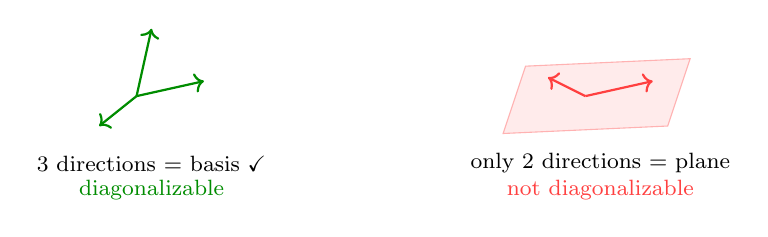
\begin{tikzpicture}[scale=0.95, every node/.style={font=\footnotesize}]
% left: 3 vectors -> basis (good)
\draw[->, green!55!black, thick] (0,0) -- (0.9,0.2);
\draw[->, green!55!black, thick] (0,0) -- (0.2,0.9);
\draw[->, green!55!black, thick] (0,0) -- (-0.5,-0.4);
\node at (0.2,-0.9) {$3$ directions $=$ basis \checkmark};
\node[green!55!black] at (0.2,-1.25) {diagonalizable};
% right: 2 vectors -> plane (bad)
\begin{scope}[xshift=6cm]
\draw[fill=red!8, draw=red!30] (-1.1,-0.5) -- (1.1,-0.4) -- (1.4,0.5) -- (-0.8,0.4) -- cycle;
\draw[->, red!75, thick] (0,0) -- (0.9,0.2);
\draw[->, red!75, thick] (0,0) -- (-0.5,0.25);
\node at (0.2,-0.9) {only $2$ directions $=$ plane};
\node[red!75] at (0.2,-1.25) {not diagonalizable};
\end{scope}
\end{tikzpicture}
\end{center}

%-----------------------------------------------------------------------------
\section*{3. What is it good for? Powers become easy}

The biggest advantage: with $A = P D P^{-1}$ every \textbf{power} becomes child's play. The middle $P^{-1}P$ cancel out:
\[
A^k = (PDP^{-1})(PDP^{-1})\cdots(PDP^{-1}) = P\,D^k\,P^{-1},
\]
and $D^k$ is just the diagonal to the power $k$:
\[
D = \begin{pmatrix} \lambda_1 & 0 \\ 0 & \lambda_2 \end{pmatrix} \ \Rightarrow\
D^k = \begin{pmatrix} \lambda_1^k & 0 \\ 0 & \lambda_2^k \end{pmatrix}.
\]

\begin{merkbox}[title={Application: sequences}]
A recurrence like $a_k = 3a_{k-1} + 10a_{k-2}$ is written as $v_k = M v_{k-1}$, i.e.\ $v_k = M^k v_0$. Via $M^k = P D^k P^{-1}$ you get an \textbf{explicit formula} for $a_k$ -- without computing all the intermediate terms.
\end{merkbox}

%-----------------------------------------------------------------------------
\section*{4. Parameter problems: ``for which $a$?''}

Sometimes a letter $a$ sits in the matrix. Then the eigenvalues depend on $a$, and you ask: for which $a$ is $A$ diagonalizable? \textbf{Strategy:} determine the eigenvalues (with AM) as expressions in $a$, then check the GM of the repeated eigenvalue. Usually there are only \emph{few} ``bad'' $a$ where two eigenvalues collide and an \EV{} is missing.

\begin{merkbox}[title={Two useful structures (from HW11)}]
\begin{itemize}[leftmargin=*, nosep]
    \item \textbf{$A = cI + (\text{all-ones matrix})$}: subtracting $cI$ only shifts the eigenvalues. The all-ones matrix has rank $1$ $\Rightarrow$ large eigenspace.
    \item \textbf{Rank-$1$ matrix} (all rows multiples of the same row): the eigenvalues are $\operatorname{trace}$ (once) and $0$ (otherwise). GM$(0) = n - 1$.
\end{itemize}
\end{merkbox}

\newpage

%=============================================================================
\part*{Part 2: Overview of the exercises}

\section*{Exercise 47 -- diagonalize (with HW11 data)}

We already know the three matrices from HW11 (43, 44). You start with the table (eigenvalues, AM, GM, bases) and only check GM $=$ AM:
\begin{itemize}[leftmargin=*, nosep]
    \item \textbf{(a)} all GM $=$ AM $\Rightarrow$ diagonalizable. $P =$ eigenvectors as columns, $D = \operatorname{diag}(3,3,5)$.
    \item \textbf{(b)} GM$(2) = 1 <$ AM$(2) = 2$ $\Rightarrow$ only $2$ instead of $3$ eigenvectors $\Rightarrow$ \emph{not} diagonalizable.
    \item \textbf{(c)} all GM $=$ AM $\Rightarrow$ diagonalizable. $D = \operatorname{diag}(0,6,6)$.
\end{itemize}
Instead of computing $P^{-1}$, you check $AP = PD$ -- that means, column by column, just $A v_i = \lambda_i v_i$.

\section*{Exercise 48 -- for which $a$?}

\begin{itemize}[leftmargin=*, nosep]
    \item \textbf{(a)} $A = \left(\begin{smallmatrix} a&1&1\\1&a&1\\1&1&a \end{smallmatrix}\right)$. The char.\ polynomial (Sarrus) gives eigenvalues $a-1$ (double) and $a+2$ (simple), \emph{always} distinct. And $A - (a-1)I$ is the all-ones matrix (rank $1$) $\Rightarrow$ GM$(a-1) = 2 =$ AM. So diagonalizable \textbf{for all $a$}.
    \item \textbf{(b)} $A = \left(\begin{smallmatrix} 1&2&3\\2&4&6\\a&2a&3a \end{smallmatrix}\right)$ has rank $1$ (all rows multiples of $(1,2,3)$). Eigenvalues $0$ (AM $2$, GM $2$) and $5+3a$ (trace). As long as $5+3a \neq 0$ everything has GM $=$ AM. At $a = -\tfrac{5}{3}$ the third eigenvalue is also $0$ (AM $3$), but GM stays $2$ $\Rightarrow$ \textbf{only then not} diagonalizable.
\end{itemize}

\section*{Exercise 49 -- sequence via diagonalization}

\begin{itemize}[leftmargin=*, nosep]
    \item $v_k = (a_{k+1}, a_k)^\top$, then $v_k = M v_{k-1}$ with $M = \left(\begin{smallmatrix} 3&10\\1&0 \end{smallmatrix}\right)$, so $v_k = M^k v_0$, $v_0 = (-1,4)^\top$.
    \item Diagonalize $M$: eigenvalues $5, -2$, eigenvectors $(5,1), (-2,1)$.
    \item $v_k = P D^k P^{-1} v_0$. With $P^{-1} v_0 = (1,3)^\top$ it follows that $a_k = 5^k + 3\cdot(-2)^k$.
\end{itemize}

%=============================================================================
\section*{Summary}

\begin{center}
\begin{tabular}{@{}ll@{}}
\toprule
Exercise & Result \\
\midrule
$47$ (a) & diagonalizable, $D = \operatorname{diag}(3,3,5)$ \\
$47$ (b) & \emph{not} diagonalizable (GM$(2) < $ AM$(2)$) \\
$47$ (c) & diagonalizable, $D = \operatorname{diag}(0,6,6)$ \\
$48$ (a) & for all $a \in \mathbb{R}$ \\
$48$ (b) & exactly for $a \neq -\tfrac{5}{3}$ \\
$49$ & $a_k = 5^k + 3\cdot(-2)^k$ \\
\bottomrule
\end{tabular}
\end{center}

\begin{merkbox}[title={Golden rules}]
\begin{enumerate}[leftmargin=*, nosep]
    \item Diagonalizable $\Leftrightarrow$ for every eigenvalue GM $=$ AM (enough eigenvectors for a basis).
    \item $P =$ eigenvectors as columns, $D =$ eigenvalues on the diagonal -- \emph{same order}.
    \item Check with $AP = PD$ (column by column $A v_i = \lambda_i v_i$) -- no $P^{-1}$ needed.
    \item Powers: $A^k = P D^k P^{-1}$, and $D^k$ is the diagonal to the power $k$.
    \item Parameter: only look for the few $a$ where GM $<$ AM.
    \item Sequences: pack into a vector, matrix $M^k$ via diagonalization, read off the component.
\end{enumerate}
\end{merkbox}

\end{document}
